\definecolor{ptten}{RGB}{35,35,35}
\definecolor{crossedparent}{RGB}{35,35,35}
\definecolor{globalparent}{RGB}{0,90,190}

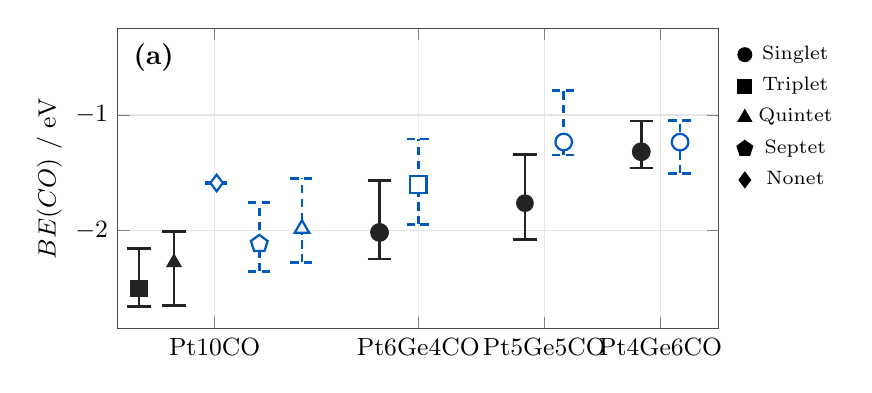
\begin{tikzpicture}
\begin{axis}[
  width=0.76\linewidth,
  height=5.4cm,
  xmin=0.45, xmax=3.55,
  ymin=-2.85, ymax=-0.25,
  xtick={0.95,2.00,2.65,3.25},
  xticklabels={\ce{Pt10CO},\ce{Pt6Ge4CO},\ce{Pt5Ge5CO},\ce{Pt4Ge6CO}},
  ylabel={$BE(\ce{CO})$ / eV},
  ylabel style={yshift=-2pt},
  tick label style={font=\small},
  label style={font=\small},
  grid=major,
  grid style={gray!20},
  axis line style={black!70},
  legend style={
    at={(1.02,0.98)},
    anchor=north west,
    draw=none,
    inner sep=2pt,
    row sep=1pt,
    font=\scriptsize,
    legend columns=1
  }
]
\addlegendimage{only marks,mark=*,mark size=2.5pt,black}
\addlegendentry{Singlet}
\addlegendimage{only marks,mark=square*,mark size=2.5pt,black}
\addlegendentry{Triplet}
\addlegendimage{only marks,mark=triangle*,mark size=2.8pt,black}
\addlegendentry{Quintet}
\addlegendimage{only marks,mark=pentagon*,mark size=3.0pt,black}
\addlegendentry{Septet}
\addlegendimage{only marks,mark=diamond*,mark size=2.8pt,black}
\addlegendentry{Nonet}
% Each vertical bar shows the minimum--maximum interval and each marker the
% mean over all Pt sites represented by the corresponding series. Horizontal
% offsets are used only for readability.
% Crossed-parent Pt10: triplet and quintet.
\addplot[ptten,line width=1.0pt] coordinates {(0.56,-2.657) (0.56,-2.156)};
\addplot[ptten,line width=1.0pt] coordinates {(0.50,-2.657) (0.62,-2.657)};
\addplot[ptten,line width=1.0pt] coordinates {(0.50,-2.156) (0.62,-2.156)};
\addplot[only marks,mark=square*,mark size=3.0pt,ptten] coordinates {(0.56,-2.501)};
\addplot[ptten,line width=1.0pt] coordinates {(0.74,-2.645) (0.74,-2.010)};
\addplot[ptten,line width=1.0pt] coordinates {(0.68,-2.645) (0.80,-2.645)};
\addplot[ptten,line width=1.0pt] coordinates {(0.68,-2.010) (0.80,-2.010)};
\addplot[only marks,mark=triangle*,mark size=3.0pt,ptten] coordinates {(0.74,-2.276)};
% Original Pt10 global-minimum parent: nonet, septet, and quintet.
\addplot[globalparent,densely dashed,line width=1.0pt] coordinates {(0.96,-1.595) (0.96,-1.580)};
\addplot[globalparent,densely dashed,line width=1.0pt] coordinates {(0.90,-1.595) (1.02,-1.595)};
\addplot[globalparent,densely dashed,line width=1.0pt] coordinates {(0.90,-1.580) (1.02,-1.580)};
\addplot[only marks,mark=diamond*,mark size=3.0pt,globalparent,
  mark options={fill=white,draw=globalparent,line width=0.8pt}] coordinates {(0.96,-1.588)};
\addplot[globalparent,densely dashed,line width=1.0pt] coordinates {(1.18,-2.353) (1.18,-1.755)};
\addplot[globalparent,densely dashed,line width=1.0pt] coordinates {(1.12,-2.353) (1.24,-2.353)};
\addplot[globalparent,densely dashed,line width=1.0pt] coordinates {(1.12,-1.755) (1.24,-1.755)};
\addplot[only marks,mark=pentagon*,mark size=3.2pt,globalparent,
  mark options={fill=white,draw=globalparent,line width=0.8pt}] coordinates {(1.18,-2.114)};
\addplot[globalparent,densely dashed,line width=1.0pt] coordinates {(1.40,-2.275) (1.40,-1.547)};
\addplot[globalparent,densely dashed,line width=1.0pt] coordinates {(1.34,-2.275) (1.46,-2.275)};
\addplot[globalparent,densely dashed,line width=1.0pt] coordinates {(1.34,-1.547) (1.46,-1.547)};
\addplot[only marks,mark=triangle*,mark size=3.0pt,globalparent,
  mark options={fill=white,draw=globalparent,line width=0.8pt}] coordinates {(1.40,-1.982)};
% Pt6Ge4: crossed-parent singlet and GM-parent triplet.
\addplot[crossedparent,line width=1.0pt] coordinates {(1.80,-2.246) (1.80,-1.567)};
\addplot[crossedparent,line width=1.0pt] coordinates {(1.74,-2.246) (1.86,-2.246)};
\addplot[crossedparent,line width=1.0pt] coordinates {(1.74,-1.567) (1.86,-1.567)};
\addplot[only marks,mark=*,mark size=3.2pt,crossedparent] coordinates {(1.80,-2.016)};
\addplot[globalparent,densely dashed,line width=1.0pt] coordinates {(2.00,-1.947) (2.00,-1.207)};
\addplot[globalparent,densely dashed,line width=1.0pt] coordinates {(1.94,-1.947) (2.06,-1.947)};
\addplot[globalparent,densely dashed,line width=1.0pt] coordinates {(1.94,-1.207) (2.06,-1.207)};
\addplot[
  only marks,mark=square*,mark size=3.0pt,globalparent,
  mark options={fill=white,draw=globalparent,line width=0.8pt}
] coordinates {(2.00,-1.600)};
% Pt5Ge5: crossed parent and GM parent.
\addplot[crossedparent,line width=1.0pt] coordinates {(2.55,-2.076) (2.55,-1.342)};
\addplot[crossedparent,line width=1.0pt] coordinates {(2.49,-2.076) (2.61,-2.076)};
\addplot[crossedparent,line width=1.0pt] coordinates {(2.49,-1.342) (2.61,-1.342)};
\addplot[only marks,mark=*,mark size=3.0pt,crossedparent] coordinates {(2.55,-1.763)};
\addplot[globalparent,densely dashed,line width=1.0pt] coordinates {(2.75,-1.346) (2.75,-0.788)};
\addplot[globalparent,densely dashed,line width=1.0pt] coordinates {(2.69,-1.346) (2.81,-1.346)};
\addplot[globalparent,densely dashed,line width=1.0pt] coordinates {(2.69,-0.788) (2.81,-0.788)};
\addplot[only marks,mark=*,mark size=3.0pt,globalparent,
  mark options={fill=white,draw=globalparent,line width=0.8pt}] coordinates {(2.75,-1.234)};
% Pt4Ge6: crossed parent and GM parent.
\addplot[crossedparent,line width=1.0pt] coordinates {(3.15,-1.459) (3.15,-1.052)};
\addplot[crossedparent,line width=1.0pt] coordinates {(3.09,-1.459) (3.21,-1.459)};
\addplot[crossedparent,line width=1.0pt] coordinates {(3.09,-1.052) (3.21,-1.052)};
\addplot[only marks,mark=*,mark size=3.2pt,crossedparent] coordinates {(3.15,-1.318)};
\addplot[globalparent,densely dashed,line width=1.0pt] coordinates {(3.35,-1.506) (3.35,-1.046)};
\addplot[globalparent,densely dashed,line width=1.0pt] coordinates {(3.29,-1.506) (3.41,-1.506)};
\addplot[globalparent,densely dashed,line width=1.0pt] coordinates {(3.29,-1.046) (3.41,-1.046)};
\addplot[only marks,mark=*,mark size=3.0pt,globalparent,
  mark options={fill=white,draw=globalparent,line width=0.8pt}] coordinates {(3.35,-1.235)};
\node[anchor=north west,font=\bfseries] at (rel axis cs:0.01,0.98) {(a)};
\end{axis}
\end{tikzpicture}
